\documentclass[a4paper]{article}

% Typesetting
%\usepackage{mathpazo}
\usepackage{geometry}
\usepackage{hyperref}
\usepackage{setspace}
\usepackage[activate={true,nocompatibility},final,tracking=true,kerning=true,spacing=true,factor=1100,stretch=20,shrink=20]{microtype}
\microtypecontext{spacing=nonfrench}
\hyphenpenalty=5000
\tolerance=1000
\usepackage{listings}
\usepackage{pdfpages}
\usepackage{tabularx} % in the preamble
\usepackage{setspace}


% Graphics
\usepackage{graphicx}
\graphicspath{{./images/}}

% Tables
\usepackage{booktabs}

% Utility
\usepackage{url}
\usepackage{amssymb}
\usepackage{amsmath}
\usepackage{amsfonts}
\usepackage{subfigure}
\usepackage{algorithm}
\usepackage{algorithmic}
\usepackage{enumerate}
\usepackage{eulervm}
\usepackage{tikz}
\usepackage{xcolor}
\usepackage{color}
\usepackage{todonotes}

\renewcommand{\algorithmiccomment}[1]{\hfill// \textit{#1}}

\usepackage{framed, color}
\definecolor{shadecolor}{rgb}{0.8, 0.9, 1.0}

% Science Units
\usepackage{textcomp}
\usepackage[]{siunitx}
\sisetup{tophrase=--}
\sisetup{repeatunits=false}
\usepackage{latexsym}

% Bibliography (Use \citep)
\usepackage[]{natbib} %numbers
\setlength{\bibsep}{3.5pt}

\begin{document}

% Title Page
\newgeometry{margin=3cm}
\thispagestyle{empty}
\begin{center}
% StarFish Logo

\includegraphics[width=\linewidth]{logo_starfish_project}\\\vspace{1cm}

% Subtitle
{\large
Finding implicitly related items based on semantic similarities and metadata in a non-hierarchical network of documents
}\\\vspace{0.5cm}

% Authors
\begin{tabular*}{0.8\linewidth}{@{\extracolsep{\fill}}lcr}
& \textbf{Authors} & \\
\hline
R. van Ginkel 	& J. Peters 	& L. Weerts \\
\end{tabular*}
\\\vspace{2cm}
% Company
Project commissioned by \emph{Perceptum B.V.}\\\vspace{1cm}

% Supervisors
\textbf{Supervisors}\\
\begin{tabular}{r|l}
Academic Supervisor & Raquel Fernandez \\
Company Supervisors & Robrecht Jurriaans \\
& Sander Latour \\
& Wijnand Baretta
\end{tabular}


% UvA
\vfill
\today\\
Universiteit van Amsterdam

\end{center}
\restoregeometry

\clearpage

% Front Matter
\begin{abstract}

\end{abstract}

\tableofcontents
\clearpage

% Main Matter
% The introduction (dah)

% DO NOT COMPILE THIS FILE DIRECTLY!
% This is included by the other .tex files.

\section{Introduction}

This report describes the results of the Second Year's project for the Perceptum team. The project focused on creating a \emph{document link recommender system} to the StarFish website. 

StarFish, one of the products of Perceptum, is a website that aims to share knowledge about the education domain by means of a connected graph. People from all around the world should get access to this knowledge graph in a simple, personalized manner. The nodes in this graph are documents and they are connected with links. These documents can be of all sorts of types - e.g. a good practice, information, a question. Each document has a set of tags associated with it, which describe the different aspects of educational innovation. StarFish is community-driven: both the content of the documents as the links between documents are determined by the users of StarFish. The drawback of a community-driven knowledge graph is that not all the users have complete knowledge the entire document base. Therefore, many links will not be made because the users are unaware of the documents that they could link to. A possible solution could be to make use of administrators, which can devote more time in getting to know all the documents. However, that approach has two main drawbacks. First of all, this would mean that some central authority determines whether or not two documents should be linked. This is not in line with the idea of a community-driven knowledge base. Secondly, if the knowledge base grows even further, it becomes impossible for an administrator to keep track of all documents. Imagine one person having to link all pages on Wikipedia - an impossible job. 

In order to overcome the problem of linking documents in a large knowledge base, this process should be automated. This project focuses on the automatization of connecting documents within Starfish. Though ideally these connections should be made completely automatic, a first step would be to create a recommendation system. When a user adds a new document, he or she can choose from a list of proposed documents the documents he or she deems relevant. This means that the recommender system does not have to work perfect, but should work reasonably well enough. Defining 'well enough', however, is also a part of this project. Thus, the product vision of the system can be described by the following:

\begin{shaded}
\textbf{{\large Product vision:}} \vspace{0.4\baselineskip} \hrule
 	\begin{tabular}{ll}
 		& \\
 		{\bf For} & StarFish users \\
 		{\bf who} & search for and edit knowledge in starfish\\
 		{\bf the} & starfish document linker \\
 		{\bf is} & a starfish core system addition\\
 		{\bf that} & finds related documents\\
 		{\bf unlike} & moderated or individual linking\\
 		{\bf our} & product uses algorithms and data to suggest document links 
	\end{tabular}
\end{shaded}


Within the time span of this project multiple ways of recommending links between documents have been explored. The results of these explorations will be discussed in this report. 

% Domain (what are we dealing with and why is it non-trivial

% DO NOT COMPILE THIS FILE DIRECTLY!
% This is included by the other .tex files.

\section{Domain}
The Starfish website aims to be a platform for educators where educational innovations and projects can be shared. Because many teachers have different vocabulary and diverse questions, a strict hierarchical structure of the shared content becomes a problem. Starfish tries to overcome this by structuring it's knowledge base in a non-hierarchical manner. There are sub communities within Starfish which gives learners the opportunity to share knowledge that is specific to their faculty or institution. 

The knowledge base itself consists of one big set of entities. These entities are called documents. Currently, the Starfish knowledge graph contains 240 documents. These documents can be of a variance of types. Each document in this graph is of one of the following types: Information, Glossary, Question, Good Practice, Project, Person or Event. Documents have an author, title, text, tags and links. The Person type is an exception on that and has a name-field instead of title and a about-field instead of text. Some document types have different optional fields like `headline' for good practices and projects. The graph is structured by directional links between documents.  On average a document x outgoing links, and x incoming links.

Each document in the knowledge base has a set of tags assigned to it, based on the different aspects of educational innovation the document covers. On average a document has x tags. Glossaries are special types of documents, as they are description for tags. This means that it is unnecessary for the link recommendation system to return Glossaries, since a glossary could better be 'linked' via assigning a tag. Because different groups use alternative names to describe concepts, tags can be aliases of each other. For this project, aliased tags are regarded as one single tag. Of the 210 tags the current system contains, x unique tag concepts can be distinguished of which x\% have a glossary. 

These numbers and properties of the system give some insight into the current state of the dataset and possible solutions. The major part of Starfish data is text-based, so semantical document analysis could be performed with standard text processing techniques. The tags of documents could also give insight into the semantics of the documents. Additionally, the links that are currently in Starfish can be used as guidelines on when documents should be linked and when not. Though Starfish aims to be user-driven, it is unfeasible to make the linking user driven with the current dataset. Such an approach could focus on a reinforcement learning system, that learns of the the opinion of users by means of a voting procedure. However, the data needed for this is simply not available. 


% Theory (how could this problem theoretically be solved)
\section{Theory}

In solving the linking problem, one must find a way to compare different
documents based on their linkability with a newly added documents.
Computationally, this can be done by creating document descriptors -- vectors
that the describe the features of a document in some way. Given the Starfish
domain, this can be done in a tag-based and text-based approach towards
creating document descriptors. This section will elaborate the background of
the descriptor-based approach. 

\subsection{Text-based descriptors: bag of words and TF-IDF}
One way of capturing the semantic similarity of two text document is by
comparing the TF-IDF values of their contents. If two documents cover the same
subject(s), they are likely to contain similar keywords. To capture this
similarity, the documents can be transformed into a list of all words that are
present within that text. This is called a bag-of-words representation. Instead
of counting the frequency of each word within a document, the more
sophisticated Term Frequency-Inversed Document Frequency value can be used.
TF-IDF is a statistic that reflects the importance of a word in a document
within a corpus and can be calculated as follows:

\begin{align}
\textrm{tf}(t,d) = 0.5 + \frac{0.5 \times {f}(t, d)}{\max\{{f}(w, d):w \in d\}}\\
\textrm{idf}(t, D) =  \log \frac{N}{|\{d \in D: t \in d\}|}\\
\textrm{tfidf}(t,d,D) = \textrm{tf}(t,d) \times \textrm{idf}(t, D)
\end{align}

The TF-IDF induces a trade off between the term frequency, the number of times
a word appears in a document, and the inverse document frequency, the inverse
of how often a word is used in the entire corpus. Words such as 'and', 'or',
and 'of' will have a high term frequency within a document. However, their
inverse document frequency will be very low, since they occur very often within
the entire corpus. Infrequent used words such as Starfish are less likely to
occur within a corpus, so if they do occur often within one particular document
the TF-IDF value will be high. 

\subsection{K-Nearest Neighbor}
After creating the document descriptors as described in the previous section
all document lay in a specific vector space. For each of this vectors we
can compute a distance using a specific distance measure. The $K$-Nearest
Neighbor algorithms selects the $K$ document descriptors that have the lowest
distance. In other words the $K$ vectors that are most similar in the given
vector space. See algorithm~\ref{algo:knn} for pseudocode of the $K$-Nearest
Neighbir algorithm.

\begin{algorithm}                      
  \caption{$K$-Nearest Neighbor}      
  \label{algo:knn}
  \begin{algorithmic}

    \STATE docs $=$ Vector document descriptors.
    \STATE dist $=$ Vector document distance metric.
    \STATE d $=$ Document to find neighbors of.
    \STATE $\delta$ = []
    \FOR{doc $\in$ docs} 
      \STATE $\delta \Leftarrow$ (doc, dist(d, doc))
      \COMMENT{Compute distance with every document}
    \ENDFOR
    \STATE sorted $=$ sort(delta)
    \COMMENT{Sort from lowest to highest distance}
    \RETURN sorted$[0\ldots K]$
    \COMMENT{Return $K$ first documents}
  \end{algorithmic}
\end{algorithm}

\subsubsection{Distance Metric}
As discussed before the $K$-Nearest Neighbor algorithm uses a distance metric
to compute the distance between two document descriptors in a given vector
space. A distance metric or simply called the distance is a function $d$ that 
maps two documents descriptors $X$ and $Y$ to the real numbers (\ref{distmap}).
\begin{align}
  d : X \times Y \mapsto \mathbb{R} \label{distmap}
\end{align}
This function $d$ at least satisfies the following conditions for the documents
$X$, $Y$ and $Z$.
\begin{align*}
  1.\ \ \ & d(X,Y) \geq 0 \\
  2.\ \ \ & d(X,Y) = 0\  \text{if and only if $X=Y$} \\
  3.\ \ \ & d(X,Y) = d(Y,X) \\
  4.\ \ \ & d(X,Z) \leq d(X,Y) + d(Y,Z)
\end{align*}

A set of distance metrics is discussed in the following paragraphs. Each are
discussed for a documents with documents descriptor  $q = [q_1, q_2, \ldots,
q_n]^T$ and $p = [p_1, p_2, \ldots p_n]^T$.


\paragraph{Euclidean distance}
The euclidean distance metric is a generalization of the pythagorean metric to
higher dimensions. The euclidean distance is the ruler distance or in other 
words the distance between the two heads of each vector.

\begin{align*}
  d_{\text{euclid}}(q,p) &= \sqrt{(q_1 - p_1)^2 + (q_2 - p_2)^2 + \cdots + (q_n - p_n)^2}  \\
                         &= \sqrt{\sum_{i=1}^n (q_i - p_i)^2} \\
                         &= \sqrt {(q-p) \cdot (q-p)} \\
                         &= || q - p ||
\end{align*}
This shows that the euclidean distance is the norm of the vector $p-q$ or 
$q-p$ (as $d(q,p) = d(p,q)$). This makes sense as the euclidean distance
is the distance between the two vectors. An illustration of this is given in
figure~\ref{fig:euclid}

\begin{figure}[h!]
 \center
 \begin{tikzpicture}[scale=2.5]
   \fill [white] (-.5,1.75) rectangle (1.5, -.75);
   \draw[step=0.5,gray!40,thin] (-.5,-.5) grid (1.5,1.5);

   % Draw axes
   \draw [<->] (0,1.5) node (yaxis) [above] {$y$}
     |- (1.5,0) node (xaxis) [right] {$x$};
 
   \draw [->, thick, red] (0,0) -- (0.5,0.5) node [above right] {$p$};
   \draw [->, thick, blue] (0,0) -- (0.25,1.0) node [above right] {$q$};

   \draw [<->, thick, gray] (0.5,0.5) -- (0.375, 0.75) node [above right] {$d$} -- (0.25,1.0);
 
   % \draw [->] (0.4, 0) arc (0:20:0.4) node [above right,inner sep=0pt] {\small{$\theta$}} arc (20:45:0.4);
 
   \draw (0,0) node [below left] {$O$};
\end{tikzpicture}

 \caption{The euclidean distance $d$ between two document descriptors $p$ and $q$.}
 \label{fig:euclid}
\end{figure}

\paragraph{Cosine distance} The cosine distance measures the cosine of the
angle $\varphi$ between two document descriptors. The intuition of this metric
is that a document `word$_1$ word$_2$' and `word$_1$ word$_1$ word$_2$
word$_2$' probably are very similar as only the word frequencies differ.
However, the euclidean distance does compute a distance $> 0$. The cosine
distance computes the angle between two documents. This is shown visualy in
figure~\ref{fig:cosine}. In this example the descriptors would point in the
exact same direction only the second descriptor is longer.  This results in a
cosine of zero, which means an exact match. The values in the vectors will
never take a value $< 0$ because a word can not occur less then zero times.
Because of this the values of the cosine of the angle between two descriptors
will range between $0$ and $1$. Where 0 means no match at all and 1 is an exact
match. Therefore the cosine distance is defined as:
\begin{align*}
  d_\textrm{cos}(q,p) = |\cos(\varphi) - 1|
\end{align*}
where $\varphi$ is the angle between $q$ and $p$. Given that $q \cdot p = ||q||
\,||p|| \cos(\varphi)$ we can easily compute the $\cos(\varphi)$. This results
in the definition of the cosine distance metric in equation~\ref{eq:cos}. It is
very efficient to compute the cosine distance on sparse vectors as only the
non-zero values are important for the computation.

\begin{align}
  d_\textrm{cos}(q,p) = \left| \frac{q \cdot p}{||q||\,||p||} - 1\right| \label{eq:cos}
\end{align}

\begin{figure}[h!]
 \center
 \begin{tikzpicture}[scale=2.5]
   \fill [white] (-.5,1.75) rectangle (1.5, -.75);
   \draw[step=0.5,gray!40,thin] (-.5,-.5) grid (1.5,1.5);

   % Draw axes
   \draw [<->] (0,1.5) node (yaxis) [above] {$y$}
     |- (1.5,0) node (xaxis) [right] {$x$};
 
   \draw [->, thick, red] (0,0) -- (0.5,0.5) node [above right] {$p$};
   \draw [->, thick, blue] (0,0) -- (0.25,1.0) node [above right] {$q$};

   \draw [->, gray] (0.25, 0.25) arc (45:64:0.4) node [above right,inner sep=0pt] {\small{$\varphi$}} arc (64:72:0.4);

   \draw (1,1) node [above] {$d = |\cos(\varphi)-1|$};
 
   \draw [gray] (0,0) node [below left] {$O$};
\end{tikzpicture}

 \caption{The cosine distance $d$ between two document descriptors $p$ and $q$.}
 \label{fig:cosine}
\end{figure}

\paragraph{Bhattacharyya distance} The feature vectors used to represent documents can
also be seen as unordered histrograms. A way to compare histrograms is the
Bhattacharyya distance metric. The Bhattacharyya metric is used to compute
the similarity of two discrete or continuous probability distributions. The 
metric ranges from 0 tot 1 where 0 is a perfect match. The Bhattacharyya 
distance metric is defined as:
\begin{align}
  d_B (q,p) = \sqrt{1 - \frac{1}{\sqrt{\overline{q}\,\overline{p}n^2}}\sum_{i=1}^n \sqrt{q_ip_i}}
\end{align}
where $\overline{q} = \frac{1}{n}\sum_{j=1}^n q_j$ and $n$ the number of
elements in each of the vectors.

\paragraph{Intersection} Another histrogram similarity metric is the histogram
intersection. The histogram intersection \citep{swain1991color} was originaly
introduced in the computer vision field and is defined in as shown in
equation~\ref{eq:intersection}
\begin{align}
  d_\textrm{int}(q,p) = \sum_{i=1}^n \min(q_i, p_i) \label{eq:intersection}
\end{align}
In the computer vision domain this results in the number of pixels that have
the same color. For the document descriptors used in this case this comes
down to the weights the two documents have in common. In other words when
two documents that have high weights for the same words the total will be
higher then when two documents have hight weights for different words. This
measure does not satisfy the four conditions for a distance metric, however
it may still be useful in the document similarity domain.

\paragraph{Cross-correlation} Finally a method often used to compute the
similarity between histograms is the cross-correlation. Correlletation measures
the dependence between two sample sets. However, as shown
\todo[inline]{Show that correlations is equivalent to cosine distance?}


% What have we actually implemented
\section{Product overview}

The product created in this project is a python program takes a set of
documents and a new document and returns the subset of documents that should be
linked with the new document. For this, a descriptor-based approach was used,
which consists of three steps. Firstly, each of the documents is transformed
into a descriptor. Secondly, a ranking is made of all documents based on the
similarity of the document descriptors and the descriptor of the new added
document. This was done using the Nearest Neighbor algorithm with several
distance metrics. Lastly, an algorithm chooses the proper amount of proposed
links that must be returned.

We will now discuss each of these parameters, since these will give more
insight into the approach that was chosen to solve the problem. For the
performance of the different parameters we refer to the experiment section. 

\subsection{Vectorizer}
The first step is to create document descriptors, which is done by algorithms that we call \emph{vectorizers}. Two main paths have been explored: transformation based on text and transformation based on tags.

\subsubsection{Text-based transformation}
\begin{description}
\item [Textvectorizer] The text-based vectorizers use the textual content of the documents and are therefore generally applicable to knowledge bases that contain text-based documents. The textual content is first transformed into a bag of words. Then, based on all the documents in the knowledge base, the \emph{TF-IDF} value is calculated for each of the words in the bag of words.  

\item[Weighted\_textvectorizer] The weighted textvectorizer is implemented as an extension of the textvectorizer. First, all descriptors of the documents are calculated similarly as in the textvectorizer. Then each document descriptor is increased with the sum of the descriptors of the document it is linked to itself, decreased by some weight. This captures the idea that if a new document resembles some of the documents that are linked to one particular document, it is more likely to be linked to this particular document. 
\end{description}

\subsubsection{Tag-based transformations}
\begin{description}
\item[Simple\_tag\_similarity] The tag-based transformations are more StarFish specific, since they make use of the tags that are assigned to the documents. A tag is a keyword that describes a topic/term that is important for that document. For example, 'Online Support and Online Assessment for Teaching and Learning Chemistry' is tagged with 'chemistry', 'e-learning' and 'assessment'. The simple tag similarity vectorizer creates a vector where each value indicates whether or not one particular tag is assigned to the document. 

\item [Tag\_smoothing] The tag smoothing vectorizer uses the co-occurence of tags in estimating document similarity. Even though tags might not co-occur on any document in the data set, they can still provide information about each other. For example, the dataset consists of documents with associated tags like $\{\{t_1, t_2\}, \{t_1, t_3\}\}$. From the co-occurence it does not follow that $t_2$ and $t_3$ are related, however by transitivity with $t_1$ we want to create a small implicit link between $t_2$ and $t_3$. The tag smoothing method does this based on work from \citet{zhou2011web}.

\item [Glossaries\_of\_tags] Another way of capturing tag similarity is by using tag Glossaries. They can be used by applying a text-based transformation on the glossaries to indicate the similarity between tags. Thus, glossaries\_of\_tags can be seen as a hybrid form of the tag and text-based approaches, where the glossary of a tag is turned into a TF-IDF bag of words. The document descriptor consists of the sum of vectors of each of its tags. 

\item [Weighted\_tag\_vectorizer] This is an extension of glossaries of tags.
  In the original glossaries of tags, it is assumed all tags contribute the
  same amount of information to a document's links. In practice some tags
  provide more information than others. If a certain tag is on nearly all
  documents in the dataset, it does not provide a lot of insight into linking
  new documents. In contrast a tag which is only attached to a small subset of
  documents is much more informative. The weighted tag vectorizer creates
  descriptors by summing the tag vectors with a weight based on the frequency
  of that tag in the dataset. The intuition for this is the same as that
  of the TF-IDF bag of words approach for creating vector representations
  of a text.
\end{description}

\subsection{Distance}
A ranking is created using the Nearest Neighbor algorithm that sorts the
document descriptors based on their distances with the newly added document.
The following five distance metrics were implemented, these are discussed
in section~\ref{sec:metrics}

\begin{itemize}
\item Eucledian
\item Cosine
\item Bhattacharyya
\item Correlation
\item Intersection
\end{itemize}

The cosine distance is the default value, since that one seems to perform the
best on the Starfish knowledge graph based on our experiments. 
More on this in section~\ref{sec:experiments}. \todo{Klopt het nog wel steeds dat deze het beste is?}

\subsection{StarFish specific adaptations: Bayesian weighting}
Both the tag-based and text-based approaches use some kind of 'semantic similarity' - the similarity of tags or text. However, except for the weighted text vectorizers, no information about possible links is used. For example, the text on a person's profile might be similar to other persons, but within Starfish a person is almost never linked to another person. In the Bayesian weighted vectorizer this is captured by weighting the vectors with the probability that two documents are linked together given their tags:
\begin{align}
\nonumber P(D_a \rightarrow D_b | t)
\end{align}
Thus, the weight of a tag within a vector is equal to the chance that given this particular vector, a document of type a (the type of the newly added document) and a document of type b (equal to the type of proposed link) are linked. The inverse of this probability is multiplied with the distances that come from Nearest Neigbor in order to enlarge the distance of proposed links that are unlikely given the Starfish knowledge base. 
\todo[inline]{Rewrite section to show steps and computations}

\subsection{Threshold value}
The next step in the pipeline is to determine how many of the nearest neighbours should be returned. Depending on the application of the Starfish document linker, the desired number might vary. If one wants to immediately link the results, the certainty for relatedness should be high. If the links are presented to a user which can approve or reject them, the relatedness may be lower. Currently, this is configurable by setting the threshold parameter between 0 and 1. Zero will only return the closest document, 1 will return almost all. After exploration of the dataset the default value is 0.3, which roughly returns the same amount of links which is currently average for Starfish.

\subsection{Results}
There are two ways in which the results of the document linker are reported: a JSON file and a textual performance report. The document linker saves the results for a given knowledge base to a file called `[vectorizer]\_[distance metric].json'. The proposed links can be viewed by opening \emph{view.html} from a browser and selecting the preferred json file. If the file is opened it displays a list of all the documents. Clicking on the 'content' button shows the title, text (or headline and about section in the case of Persons) of the document. Clicking on the 'links' button shows a list of titles of other documents. The grey ones indicate False Negatives: correct links that were not recalled. The green ones are correct proposed links, the red ones incorrect proposed links. The content of these documents can also be viewed. 


% Very specific explanation of each of the algorithms in the pipeline and their pro's and cons
\section{Method}

\subsection{Data preprocessing}
Starfish text content is serialized as HTML, a format which is not suitable for
calculating semantical similarity. Before processing, the data is sanitized by
removing HTML tags and entities and convert unicode characters to their closest
ASCII representation.

The raw starfish data contains tags which are aliases of other tags. During 
preprocessing all tags are replaced by their alias which have a glossary. Also, 
the current graph also contains some links which should not be returned by a 
link recommender system. Links from article to an author should be ignored as 
an author is automatically linked from the document. Links to glossaries should 
never occur, as they are linked through tags if appropriate.

After the data is sanitized, the tags are unique and the inappropriate links are 
removed, the data is ready for processing.

\subsection{Text descriptors}
\subsubsection{Textvectorizer}

The first set of vectorizers focuses on the texts of the documents. The
\emph{textvectorizer} is a very generic approach that can be used on any corpus
of textual documents. In the Starfish context, we define 'content' as the title
and text-fields of a document. The only exception on this are Persons, of which
we will use the name and about-fields. 

The textvectorizer first transforms the set of documents into a bag of words
and calculates the TF-IDF values for all words. This was done using the
TFIDFVectorizer of scikitlearn \citep{scikit-learn}.  Though the TF-IDF values
of words that are used very often should be low, common words such as 'and',
'or' and 'of' are still present in the vectors. This could be caused by the
different types of documents. For example, a Question often structured in a
less complex way than a Project description. To prevent this from happening,
the English stopwords list that comes standard with scikit learn was used to
remove these words from the document descriptors.

\subsubsection{Weighted textvectorizer}
The weighted text vectorizer is an extension of the textvectorizer that takes
into account the links of the proposed documents. The vectors of the links of a
document are added with some weight to the vectors of the documents themselves.
Intuitively, this would add semantic information about a document based on it's
links. For example, a Person is likely to write other documents about his or
her subjects of expertise. Knowing not only the biography of a Person, but also
the content he or she has added to Starfish, gives a more complete image of
what documents could be related to that Person.

The vectors of links of a document are added in a recursive way, where
documents that are linked directly have a higher weight than documents that are
linked transitively. The algorithm is displayed in figure xx.

\subsection{Tag descriptors}
\subsubsection{Simple tag vectorizer}
The tag-based approach is more Starfish specific than the text-based approach,
since it depends on the tags that are available in Starfish. The tags on
Starfish are added by the users themselves, so offer a human-based vision on
what a document is really about. The simple tag vectorizer is a very straight
forward implementation of the idea of using tags. The vectors of this
transformation consist of a binary list that tells whether or not a tag is
attached to the document. 

\subsubsection{Tag smoothing}
The tag smoothing vectorizers creates descriptors based on the tag set of a
document. A tag co-occurs with other tags in a document, we assume documents
with similar tags should be linked in Starfish. Let the frequency of occurrence
with other tags across the dataset will form a vector for each tag. The
descriptor for a document is then created by combining the occurrence vectors
for all the document's tags. Now documents with tags that occur together will
be seen as similar.

There are two reasons why one would like to smooth the tag co-occurences.
Firstly, a problem for this is that tags must occur together before the
algorithms works properly. The Starfish dataset contains a lot of tags that
only occur with a small frequency, which means the tag occurrence vector will
contain many zeros. This makes the algorithm perform bad with little data.
Secondly, two tags can describe the same concept and be connected to that
concept through a common co-occurence with another tag. Whilst they describe
the same concept and are connected to that, they are not directly linked
together. Therefore it seems feasible to perform some sort of smoothing on the
co-occurences of tags.

\citet{zhou2011web} proposed a method to cluster web documents based on tag set
similarity. This is based on a similarity between two tags as a relation
between the frequency these tags occur separate and together, as described in
equation~\ref{eq:tag_similarity}. To smooth these similarities between tags, a
tag similarity matrix $\mathcal{C}$ is constructed. Each entry $c_{i,j}$ in
this matrix can be viewed as the angle $\theta_{i,j}$ between two unknown
vectors $v_i$ and $v_j$. These vectors cover both explicit similarity and
implicit similarity \citep{park2010vector}. This transfers the problem to find
a set of linearly independent vectors $\{v_1,v_2,\ldots,v_n\}$ for which for
all $v_i \cdot v_j = \cos(\theta_{i,j})$. One must find a matrix $\mathcal{V}$
for which $V^TV = C$. This can be done by orthogonal triangularization on
$\mathcal{C}$ for which \citeauthor{zhou2011web} introduces a modified Cholesky
transform.

\begin{equation} \label{eq:tag_similarity}
s_{i,j} = \frac{f_{i,j}}{f_i + f_j - f_{i,j}}
\end{equation}


\subsubsection{Glossaries of tags}
The glossaries of tags approach is also based on the intuition that certain
tags cover overlapping concepts. Just like the simple tag vectorizer the
glossaries of tags approach exploits this intuition. In the Starfish system a
tag is expected to have a glossary; a short English description of the concept
of a tag. These glossaries contain terms and words that are descriptive for the
tag. The glossary of tags vectorizer aims to use these terms to create a
document descriptor based on the tags associated with a document. In other
words the set of

First for each tag a tag descriptor $t_i$ is created. This tag descriptor is
a TF-IDF bag of words vector created from the glossaries of each tag. These
descriptors form the basis for the document descriptors. For each document
a document descriptor $d_i$ is created by summing the tag descriptors of the
associated tags.
\begin{align}
  d_i = \sum_{j \in T(d_i)} t_j
\end{align}
where $T(d_i)$ is the set of tag indices associated with document $d_i$. This
way a document descriptor is created based on a semantic representation of
the tags associated with the document.

\subsubsection{Weighted tag vectorizer}
The weighted tag vectorizer is similar to the glossaries of tags vectorizer
discussed in the previous section. However instead of just summing the tag
descriptors an weight is used to scale the tag descriptor. This way tags that
are associated with a lot of documents don't contribute as much to the document
descriptor as tags that are only associated with a few documents. The weight
$w_t$ for each tag descriptor $t$ is based on the number of documents that the
tag is associated with. $w_t$ is defined as follows
\begin{align}
  w_{t_i} = 1 - \frac{\textrm{Number of documents associated with $t_i$}}{\textrm{Total number of documents}}
\end{align}
With this weight the weighted tag document descriptor $d_i$ can be computed
in the following way:
\begin{align}
  d_i = \sum_{j \in T(d_i)} w_{t_j}t_j
\end{align}
This vectorizer first gives extra importance to descriptive words in each of
the tag descriptors by using the TF-IDF bag of words. After this more
importance is given to tags that are more descriptive using the weights. This
results in a document descriptor that has high weights for words that are
descriptive for tags that are descriptive for the document.

\subsection{Bayesian weighting}
Up to this point only the semantic similarity of documents has been taken into
account. This does however, not take the information in the current network
into account. For example the probability of a document of type information
linking to a document of type information is higher than that of the same
document linking to a document of type project. For this $P(d_i \to d_j \mid
\Sigma_{ij})$ and $P(d_i \to d_j)$ are interessting. Or in other words the
probability that two documents are linked given the number of tags they have in
common and the probability that two document of a given type are linked. These
probabilies can be estimated from the data. First it is shown how to compute
$P(d_i \to d_j \mid \Sigma_{ij})$.

\begin{align}
  P(d_i \to d_j \mid \Sigma_{ij}) &= \frac{P(\Sigma_{ij} \mid d_i \to d_j)P(d_i \to d_j)}{P(\Sigma_{ij})} \\
  P(\Sigma) &= \frac{{D_\Sigma \choose 2}}{{|D| \choose 2}} \\ 
  P(\Sigma \mid d_i \to d_j) &= \frac{\textrm{Number of links that have $\Sigma$ tags in common}}{|L|} \\
  P(d_i \to d_j) &= \frac{|L|}{{|D| \choose 2}}
\end{align}
Where $L$ is the set of all links and $D$ is the set of all documents.
$\Sigma_{ij}$ is the number of tags that document $d_i$ and $d_j$ have in
common. As is shown above $P(d_i \to d_j)$ is computed as a uniform probability
for all documents. However this can also be computer while taking the document
types into account. This is computed next:
\begin{align}
  P(d_i \to d_j) &= \frac{|L|}{{|D| \choose 2}}
\end{align}
These probabilities will be used to scale the distances that are
computed by the nearest neighbor algorithm. Because the distances for documents
that have a high probability should be low therefore the final distances are
computed in the following way:
\begin{align}
  d_i = (1 - P(d_i\to d_j \mid \Sigma_{ij})) \times (1-P(d_i \to d_j)) \times \delta_i
\end{align}
where $\delta_i$ is the distance as computed by the nearest neighbor algorithm
and $d_i$ the final distance that is used to select the proposed documents to
be linked. This may seem a rather simple statistical model, however due to the
limited set of items in the dataset it is very hard to learn a more complicated
model.

\subsection{Thresholds}
After creating the descriptors for a document and finding a new document's
nearest neighbors, a subpart of those links needs to be returned by the linker
application. An average document in Starfish has x links. To create a dynamic
threshold which returns similar a similar amount of documents, a document from
the Starfish data is extracted and then to re-inserted to test the number of
links the system returns to the number of links the document had in the
original system. Figure~\ref{fig:link_histogram} shows the distribution of
outgoing links in the current network.

\begin{figure}[h]
\centering
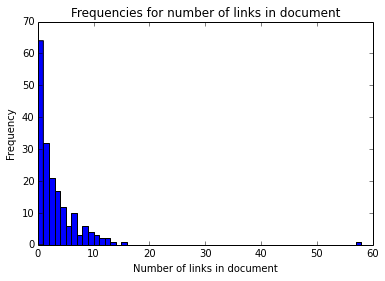
\includegraphics[width =0.45\textwidth]{images/link_histogram}
\caption{The frequency of outgoing links in Starfish documents}
\label{fig:link_histogram}
\end{figure}

The the threshold should depend on multiple factors which mostly depend on the setting in which the document linker will be used. Two major factors determine how the threshold should work.
\begin{enumerate}[1.]
	\item The degree of certainty we expect from the returned documents.
	\item The maximum number of documents that should be returned for a specific application.
\end{enumerate}
If the system is used to directly create the links into the Starfish system, the first aspect is very important. Only documents with a very high degree of linking certainty should then be returned, the amount should be based on the contents of the current system. If the system will be used to create recommendations which a user must accept or reject, the first aspect becomes less important and the system should return an amount of links which can quickly be reviewed by users. To ensure the flexibility for choice of algorithm and integration of the application, the threshold algorithm will contain a configurable parameter.

When adding a document to Starfish, it is assumed that there is always at least one related document. Based on the distance of the nearest neighbor for the new document, the index of a and the configurable parameter, the threshold is defined as in equation~\ref{eq:thresh}. In this equation, $\alpha$ is the configurable parameter, $m$ is the number of documents returned by the nearest neighbor algorithm, $d_0$ is the distance to the closest document, $\frac{m - n}{m}$ is a factor that ensures the maximum allowed distance decreases for documents ranked further away. This is based on the differences between two nearest neighbors which are visualized in figure~\ref{fig:thresholds_differences}. The distances have a long tail form: the distances between the nearest neighbors is relatively large for the closest documents and smaller between the documents further away. 

\begin{equation}
t_n = \alpha (1 - d_0) \frac{m - n}{m}
\label{eq:thresh}
\end{equation}


% Overview of experiments done on the entire pipeline
\section{Experiments}
\label{sec:experiments}
\subsection{Evaluation metrics}
In order to evaluate the performance of the different algorithms, three different metrics were used. For each of these methods we hold on to the closed world assumption that if a link is not present within the given data set, it should not be a link. 

\subsubsection{Precision and recall} \todo{So, do we thrive for higher precision or higher recall?}
Precision and recall can be calculated when the complete system pipeline is used. Precision reflects the fraction of relevant documents from all proposed documents and can thus be calculated as follows:

\begin{align*}
  \textrm{precision} = \frac{|\;\textrm{relevant\;documents} \cap \textrm{retrieved\;documents}\;|}{|\textrm{retrieved\;documents}\;|}
\end{align*}

Within a recommender system, the precision indicates how sensible the proposed links seem to the user. A precision of 50\% means that if for example two links are proposed to the user, at least one of them is correct. If one strives for a high user friendliness of the system, a high precision should be pursued. 

Recall represents the fraction of relevant documents of all originally linked documents and can be calculated as follows:
\begin{align}
  \nonumber \textrm{recall} = \frac{|\;\textrm{relevant\;documents} \cap \textrm{retrieved\;documents}\;|}{|\;\textrm{relevant\;documents}\;|}
\end{align}

The recall thus gives an indication of how well the sytem covers all the documents in the knowledge base. If the main goal of the system is to make the knowledge base as complete as possible, without taking user friendliness into account, a high recall should be obtained. 

The F1-measure can be used to capture both precision and recall into one number. If precision and recall are equally important, this can be calculated in the following way:
\begin{align}
  \nonumber \textrm{F1-measure} = \frac{2*\textrm{recall}*\textrm{precision}}{\textrm{recall} + \textrm{precision}}
\end{align}

All these metrics can be unraveled into precision, recall and F1-measure per
document type to give more insight into the performance of the algorithms with
regards to different document types. 

\subsubsection{K-links}
The k-links metric is used to evaluate the algorithms, without being influenced by the threshold for the number of proposed links. For a document with a given number of correct links, it proposes the same amount of links that the document is known to have. This evaluation metric thus makes the assumption that the algorithm knows in advance how many links should be returned. By doing so, the recall and precision are equivalent since the number of relevant and retrieved document is the same. It prevents the precision from being too optimistic, which would be the case if the fixed number would be lower than the actual amount of links. It also prevents the recall for being too optimistic in the cases that the actual amount of links is lower than the fixed number of proposed links. 

The disadvantage of the k-links metric is of course that it does not take into account the certainty the algorithm has due to the distances. For example, it could be that the distance of the first two ranked documents is very small, but the distance of the third is very large. If the original document has 10 links, the system is forced to additionally return the nine documents, even though these are likely to be wrong because they have a relatively big distance. 

\begin{table}

\begin{tabular}{| l | l | l | l | l | l | l | l |}
\hline
{\bf CORRELATION} & Inf. &  Question &  Good Pr.& Project & Person &  Event & {\bf Average} \\
\hline
Textvectorizer & 20.49 & 42.02 & 30.35 & 25.41 & 5.81 & 21.42 & {\bf 19.73} \\ 
Weighted text & 21.25 & 44.82 & 30.35 & 16.04 & 5.81 & 21.43 & {\bf 19.76} \\ 
Simple tag & 21.33 & 16.67 & 69.64 & 37.81 & 14.87 & 46.83 & {\bf 21.90} \\ 
Tag smoothing & 20.95 & 21.93 & 44.64 & 31.04 & 13.59 & 46.83 & {\bf 20.78} \\ 
Glossaries of tags & 17.70 & 16.67 & 48.21 & 31.46 & 7.95 & 40.47 & {\bf 16.77} \\ 
Weighted tag & 17.70 & 16.67 & 48.21 & 31.46 & 7.95 & 40.48 & {\bf 16.77} \\ 
\hline
\\
\hline
{\bf COSINE} & Inf. &  Question &  Good Pr.& Project & Person &  Event & {\bf Average} \\
\hline
Textvectorizer & 20.49 & 40.70 & 30.36 & 25.42 & 5.81 & 21.43 & {\bf 19.49} \\ 
Weighted text & 21.67 & 44.82 & 30.36 & 16.04 & 5.81 & 21.43 & {\bf 19.90} \\ 
Simple tag & 21.21 & 16.67 & 69.64 & 37.81 & 17.53 & 46.83 & {\bf 22.80 } \\ 
Tag smoothing & 20.58 & 21.93 & 44.64 & 31.04 & 13.59 & 46.83 & {\bf 20.69} \\ 
Glossaries of tags & 18.68 & 16.67 & 48.21 & 31.46 & 10.51 & 40.48 & {\bf 18.02} \\ 
Weighted tags & 18.68 & 16.67 & 48.21 & 31.46 & 10.51 & 40.48 & {\bf 18.02} \\ 
\hline
\\
\hline
{\bf INTERSECTION} & Inf. &  Question &  Good Pr.& Project & Person &  Event & {\bf Average} \\
\hline
Textvectorizer & 4.16 & 3.51 & 10.71 & 19.06 & 0.00 & 24.21 & {\bf 4.45} \\ 
Weighted text & 4.15 & 3.51 & 10.71 & 19.06 & 0.00 & 24.21 & {\bf 4.45} \\ 
Simple tag & 4.15 & 3.51 & 10.71 & 19.06 & 0.000 & 24.21 & {\bf 4.45} \\ 
Tag smoothing & 4.15 & 3.51 & 10.71 & 19.06 & 0.00 & 24.21 & {\bf 4.45} \\ 
Glossaries of tags & 4.16 & 3.51 & 10.71 & 19.06 & 0.00 & 24.21 & {\bf 4.45} \\ 
Weighted tag & 4.15 & 3.51 & 10.71 & 19.06 & 0.00 & 24.21 & {\bf 4.45} \\ 
\hline
\\
\hline
{\bf EUCLIDEAN} & Inf. &  Question &  Good Pr.& Project & Person &  Event & {\bf Average} \\
\hline
Textvectorizer & 3.04 & 3.95 & 17.86 & 0 & 0.85 & 21.43 & {\bf 3.25} \\ 
Tag smoothing & 1.32 & 1.32 & 7.14 & 0 & 0.43 & 0 & {\bf 1.08} \\ 
Simple tag & 14.05 & 10.53  & 30.36 & 38.23 & 14.36 & 35.71 & {\bf 16.56} \\ 
Tag smoothing & 0 & 0 & 0 & 0 & 0 & 0 & {\bf 0} \\ 
Glossaries of tags & 15.64 & 10.53 & 41.07 & 31.46 & 7.95 & 40.47 & {\bf 14.75} \\ 
Weighted tags & 15.64 & 10.53 & 41.07 & 31.46 & 7.95 & 40.47 & {\bf 14.75} \\ 
\hline
\\
\hline
{\bf BHATTACHARYYA} & Inf. &  Question &  Good Pr.& Project & Person &  Event & {\bf Average} \\
\hline
Textvectorizer & 15.57 & 35.88 & 30.36 & 16.15 & 5.30 & 21.43 & {\bf 16.19} \\ 
Weighted text & 18.72 & 29.04 & 30.35 & 11.99 & 7.95 & 21.43 & {\bf 16.63} \\ 
Simple tag & - & - & - & - & - & - & {\bf -} \\ 
Tag smoothing & 4.16 & 3.51 & 10.71 & 19.06 & 0 & 24.2 & {\bf 4.44} \\ 
Glossaries of tags & 18.36 & 17.98 & 48.21 & 48.13 & 10.51 & 40.45 & {\bf 19.39} \\ 
Weighted tag & 18.36 & 17.98 & 48.21 & 48.13 & 10.51 & 40.45 & {\bf 19.39} \\ 
\hline
\end{tabular}

\caption{Performance k-link measuring of all vectorizers with each of the distance metrics per document type}
\label{klink}
\end{table}

\subsection{Text-based descriptors}
Table \ref{klink} shows the k-link values of all vectorizers, including those of the textvectorizer and the weighted-text vectorizer. The best performance of the textvectorizers is obtained by the cosine distance. This can be attributed
 to the fact that the cosine distance is independent to document length and only
 computes a similarity in document structure. In other words when a document
 has the exact same words as a seconds document but only twice as much the
 cosine similarity classifies these documents as exactly equal. As the textvectorizer
 encodes the number of word occurrences in a vector the cosine distance can 
 easily find document that use the same words frequently.

The cosine distance metric gives the best results for the text vectorizers. On average, 19.49\% and 19.59\% percent of the number of proposed links respectively are correct. The weighted text vectorizer performs a bit better, which is mainly due to an improvement in performance on information and questions.

Both textvectorizers have a low percentage correct with regards to proposing links for Persons. A further analysis shows that 76.36\% (not weighted) and 69.09\% (weighted) of the links for Persons are towards other Persons. However, within the Starfish network such links almost never occur (see table \ref{bayes_table3} for the distribution of document types within Starfish). This could explain the low performance on persons. 

Overall, both textvectorizers are slow in performance even though the corpus is small. Additionally, the the bag-of-words approach imposes a few limitations on the document linker. Firstly, it performs bad when different languages are used. Figure x shows the differences of vectors of three texts when an English document is combined with an English proposed document and a Dutch proposed document. In the case of two different languages, there are less words that the two documents have in common. If important keywords entail word such as `clickers' versus `stemsysteem', there is no way of relating the two documents. Secondly, the current StarFish network consists of mainly textual content. However, in the future this is likely to be extended with images, videos and other non-textual content. These sources should then somehow be converted to text.

Table~\ref{klink} shows the k-link values of all vectorizers, including those
of the textvectorizer and the weighted-text vectorizer. The best performance of
the textvectorizers is obtained by the cosine distance. This can be
attributed to the fact that the cosine distance is independent to document
length and only computes a similarity in document structure. In other words
when a document has the exact same words as a seconds document but only twice
as much the cosine similarity classifies these documents as exactly equal. As
the textvectorizer encodes the number of word occurrences in a vector the
cosine distance can  easily find document that use the same words frequently.

The cosine distance metric gives the best results for the text vectorizers. On
average, 19.49\% and 19.59\% percent of the number of proposed links
respectively are correct. The weighted text vectorizer performs a bit better,
which is mainly due to an improvement in performance on information and
questions. % ROBBERT, FIND SOME QUALTITATIVE EXAMPLES FOR THIS. 

Both textvectorizers have a low percentage correct with regards to proposing
links for Persons. A further analysis shows that 76.36\% (not weighted) and
69.09\% (weighted) of the links for Persons are towards other Persons (see
appendix X). However, within the Starfish network such links almost never occur
(see table~\ref{bayes_table3} for the distribution of document types within
Starfish). This could explain the low performance on persons. 

Overall, both textvectorizers are slow in performance even though the corpus is
small. Additionally, the the bag-of-words approach imposes a few limitations on
the document linker. Firstly, it performs badly when different languages are
used. Figure x shows the differences of vectors of three texts when an English
document is combined with an English proposed document and a Dutch proposed
document. In the case of two different languages, there are less words that the
two documents have in common. If important keywords include words such as
`clickers' versus `stemsysteem', there is no way of relating the two documents.
Secondly, the current StarFish network consists of mainly textual content.
However, in the future this is likely to be extended with images, videos and
other non-textual content. These sources should then somehow be converted to
text.

\subsection{Tag-based descriptors}

\subsubsection{Simple tag similarity vectorizer} 
The performance of the simple tag similarity vectorizer, as shown in
table~\ref{klink} together with the other tag vectorizers, is about 26\%
precision when measuring k-link. The unraveling per document type shows that
Question documents and Person documents perform the worst. This can be
explained by the fact that half of both Questions and Persons have zero tags.
Obviously, the simple tag vectorizer cannot deal with such documents. In fact,
almost all other Questions have only one tag. Since the simple tag vectorizer
compares vectors, it will prefer documents that also have only that particular
tag, which makes it sensitive to attaching Questions to Questions. Something
similar seems to happen with Persons, of which 50.91\% of the connections are
with other Persons.  Apparently, persons with similar expertise are tagged
similarly.  However, as mentioned with the text vectorizer, in Starfish persons
almost never refer to other persons.
Moreover, if a document is badly labeled
this can also induce problems. For example, the question `TurnitIn licence at the 
UvA' has two tags, but the simple tag similarity is unable to find both it's links because 
the link `What is TurnitIn?' is not tagged with `TurnitIn'. The text vectorizer returns both
links correctly. Good practices, events and projects perform better, 
but these document types only make up to 3.2\%, 2.7\% and 5.4\% of the
total amount of documents respectively so have less influence on the average
precision.

\subsubsection{Tag smoothing}
The performance of the simple tag vectorizer, as shown in table~\ref{klink}, is
quite similar with the results of the tag similarity. It performs worse on the
information. This is visible in the `Peer-instruction' information document, in which the tag smoothing fails to make a recommendation the simple tags do. It also
performs worse on Persons, which is visible in the `Claire McDonnell' person document. That document has more tags than average but does not return any correct links.

In the current implementation this vectorizer is relatively slow. In practice
the similarity matrix can be pre calculated and updated in batches. Due to the
transform on the tag similartity matrix, it is very hard to determine which tag
occurrences contributed to the document similarity and why some recommendations
are made. It does not seem to perform much better than the regular bag of words
tag descriptor, in \citeauthor{zhou2011web} the algorithm only starts
performing significantly better when it is presented with more tags.

\subsubsection{Glossaries of tags}
The glossaries of tags approach returns the lowest results without applying the
threshold. This could be a result of the sheer number of tags which have a glossary. For
example, the documents `Is there an English version in Tentamenlade?', `De toetscyclus' 
and `Wat is het verschil tussen Learning Analytics en TTL?' all have the 
tag `ToetsenEnToetsgestuurdLeren' and at most one other tag with a glossary. 
ToetsenEnToetsgestuurdLeren is a tag with a glossary, but that glossary is one sentence 
long. This results in weak vectors which aren't very well distinctive from other documents 
which have little tags or little tags with glossaries. The information needed to link the 
documents does not seem to be present in the current dataset.


\subsubsection{Weighted tag glossaries}
Table~\ref{klink} shows that the weighted tag vectorizer, an extension of the glossaries of tags vectorizer, performs exactly the same as the glossaries of tags vectorizer. It thus seems that applying the weights has no influence on the performance of this vectorizer. The histogram in figure~\ref{weightedtag} shows the number of tags that appear in a certain amount of documents. From this can be derived that there are many tags that almost all the tags appear in 10 documents or less. There are only a few tags that appear in a lot of documents. Thus, the influence of the weighted tag vectorizer is caused by the fact that many tags assign the same or a similar weight to vector, making it approximately the same as the glossaries of tags vectorizer.  

\begin{figure}
\center
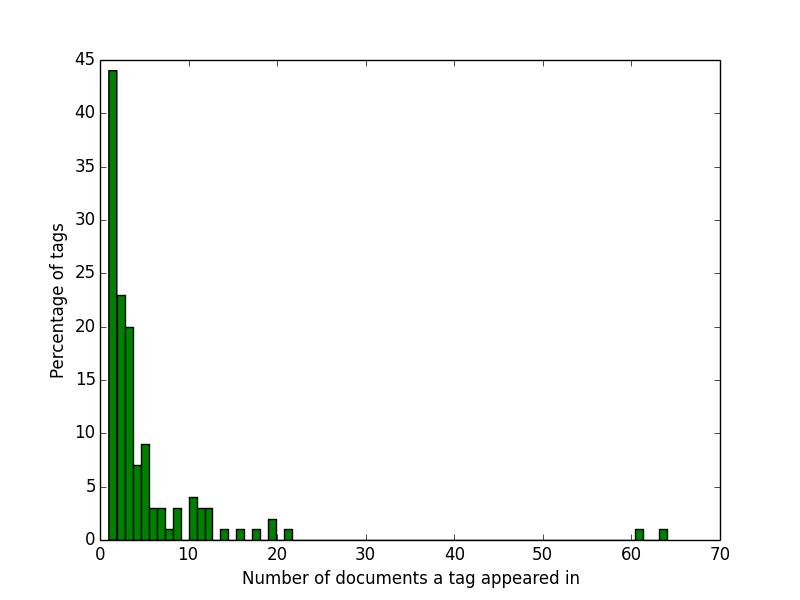
\includegraphics[width =0.6\textwidth]{images/weightedtagexplanation}
\caption{This histogram shows the number of tags that appear in a certain amount of documents. Almost all tags appear in 10 documents or less. Only a few tags are very common and these appear in about 60 different documents.}
\label{weightedtag}
\end{figure}

\subsubsection{Hybrid}
Given the previous results, the best results can be obtained if the textvectorizer and simple tag similarity are combined into one vectorizer. If a document has no tags, it will be handeled by the textvectoriser, otherwise the simple tag similarity will do this. Boht vectorizers use the cosine distance metric. The results are show in table \ref{hybrid}. This hybrid vectorizer performs significantly better than the two vectorizers themselves. 


\begin{table}[h!]
\begin{tabular}{| l | l | l | l | l | l | l | l |}
\hline
 & Inf. &  Question &  Good Pr.& Project & Person &  Event & {\bf Average} \\
\hline
Accuracy hybrid & 21.21 & 31.93 & 69.64 & 37.81 & 19.15 & 46.83 & {\bf 26.13}\\
\hline
\end{tabular}
\caption{Accuracy of a hybrid form that uses the cosine textvectorizer for questions and the correlation simple tag similarity vectorizer otherwise}
\label{hybrid}
\end{table}

\subsection{Bayesian weighting}
\begin{table}
\begin{tabular}{| l | l | l | l | l | l | l | l |}
\hline
DEVALUATION & Inf. &  Question &  Good Pr.& Project & Person &  Event & {\bf Average} \\
\hline
Textvectorizer & 0.59 & 12.63 & 0.00 & 0.00 & 0.43 & 0.00 & {\bf 2.58}\\
Weighted text vectorizer & 0.59 & 16.58 & 0.00 & 0.00 & 0.43 & 0.00 & {\bf 3.29} \\ 
Simple tag similarity & 1.18 & 10.53 & 0.00 & 4.17& 0 & 0 & {\bf 2.55}\\
Tag smoothing & 0.00 & 10.53 & 0.00 & 4.17 & 0.43 & 0.00 & {\bf 2.33}\\
Glossaries of tags & 4.61 & 13.16 & 0.00 & 6.23 & 6.41 & 0 & {\bf 6.61}\\
Weighted tags & 4.61 & 13.16 & 0.00 & 6.23 & 6.41 & 0 & {\bf 6.61}\\
\hline
\end{tabular}
\caption{Percentage correct links per vectorizer per document type after a k-link measurement whilst using tag and link devaluation NOT YET CORRECT VALUES!!!!}
\label{bayes_table1}
\end{table}

Table~\ref{bayes_table1} shows the performance of each of the vectorizers (all
with cosine distance) while applying the tag and link devaluation using the
k-link metric. It shows that the performance of all algorithms drastically
decreases when the probabilities are used to re-rank the documents. 
Table~\ref{bayes_table1}  shows the distribution of links in the simple tag
similarity vectorizer, with and without the probabilities (all based on k-link
measuring). It is clear that the links with probabilities have a sharper
distribution: the sparseness of the table shows that many types of links do not
even exist. This effect could be caused by overfitting - the data set could be
too small to calculate reliable probabilities. The preferred effect of having no
Persons link to other Persons was done correctly. However, Good Practices, for
example, are now only assigned to be a person. The vectorizer without
probabilities has a distribution that seems to be more reliable for these types
of documents. The distributions with and without probabilities can be compared
with the original distribution of links in the current Starfish knowledge base,
as shown in table~\ref{bayes_table2}.  

\begin{table}
\begin{tabular}{| l | l | l | l | l | l | l | }
\hline
DEVALUATION & {\bf Inf. }& {\bf Question }& {\bf Good Pr.} & {\bf Project }&{\bf Person }& {\bf Event}  \\
\hline
{\bf Information} & 100.00 &  0.00 &  0.00 &  0.00  & 0.00 & 0.00 \\
{\bf Question} & 11.11 &  84.44  & 0 & 2.22  & 2.22 & 0.00 \\
{\bf Good Practice} & 58.82 &  0.00  &  41.18  &  0.00  & 0.00 & 0.00 \\
{\bf Project }& 93.33 &  3.33  &  0.00  & 0.00 & 3.33 & 0.00 \\
{\bf Person} &  100.00 &  0.00 &  0.00 &  0.00  & 0.00 & 0.00 \\
{\bf Event }& 21.43 &  0.00  &  0.00 &  21.43  & 0.00 & 57.14 \\
\hline
\\
\hline
NO DEVALUATION & {\bf Inf. }& {\bf Question }& {\bf Good Pr.} & {\bf Project }&{\bf Person }& {\bf Event} \\
\hline
{\bf Information} &  21.21 & 16.67 & 69.64 & 37.91 & 17.44 & 46.83 \\
{\bf Question} & 6.67 & 35.56 &17.79 & 4.44 & 35.56 & 0 \\
{\bf Good Practice} & 41.18 & 11.76 & 17.65 & 5.88 & 5.88 & 17.65 \\
{\bf Project } & 30.0 & 16.67 & 6.67 & 13.33 & 20.00 & 13.33 \\
{\bf Person} & 30.01 & 7.27 & 3.64 & 1.81 & 50.01 & 5.45 \\
{\bf Event }& 35.71 & 0.00 & 14.29 & 28.57 & 7.14 & 14.29 \\
\hline
\end{tabular}

\caption{Percentage of links from one type (row) to another (column) for simple\_tag\_vectorizer with tag and link devaluation (above) and without (below), measured using k-link. The rows sum up to 100\%.}
\label{bayes_table2}
\end{table}

\begin{table}
\begin{tabular}{| l | l | l | l | l | l | l | }
\hline
 & {\bf Inf. }& {\bf Question }& {\bf Good Pr.} & {\bf Project }&{\bf Person }& {\bf Event} \\
\hline
{\bf Information} &  39.86 & 8.39 &4.20 &5.59 &37.76 &4.20\\
{\bf Question} & 19.72 &25.35 &12.68 &12.68 &23.94 &5.63\\
{\bf Good Practice} & 25.00 & 17.86 & 7.14 & 10.71 & 25.00 & 14.29 \\
{\bf Project } & 23.91 & 10.87 & 4.35 & 19.57 & 30.43 & 10.87 \\
{\bf Person} & 69.64 & 8.93 & 1.79 & 8.93 & 1.79 & 8.93 \\
{\bf Event }& 28.57 & 0.00 & 14.29 & 9.52 & 33.33 & 14.29\\
\hline
\end{tabular}
\caption{Percentage of links from one type (row) to another (column) for the real links in the document base}
\label{bayes_table3}
\end{table}

Figure \ref{distribution} gives insight into the reason why the probabilities
do not improve the performance. The figure shows a histogram of the percentage
of documents that have a certain probability. The left side shows the
distribution for the tag probabilities, where the red bars represent incorrect
links and the green bars show the correct ones. One would expect that a higher
percentage of correct links would be on the righthand side of the histogram,
since these should have a higher probability. However, this is clearly not the
case. On the contrary, about 75\% of the incorrect links have a chance of
0.0014, the highest probability. The link probability, shown on the right hand
side of the figure, is a bit more promising since the incorrect links are a bit
higher on the left hand side of the histogram. However, there is still no clear
difference in distribution. 

\begin{figure}
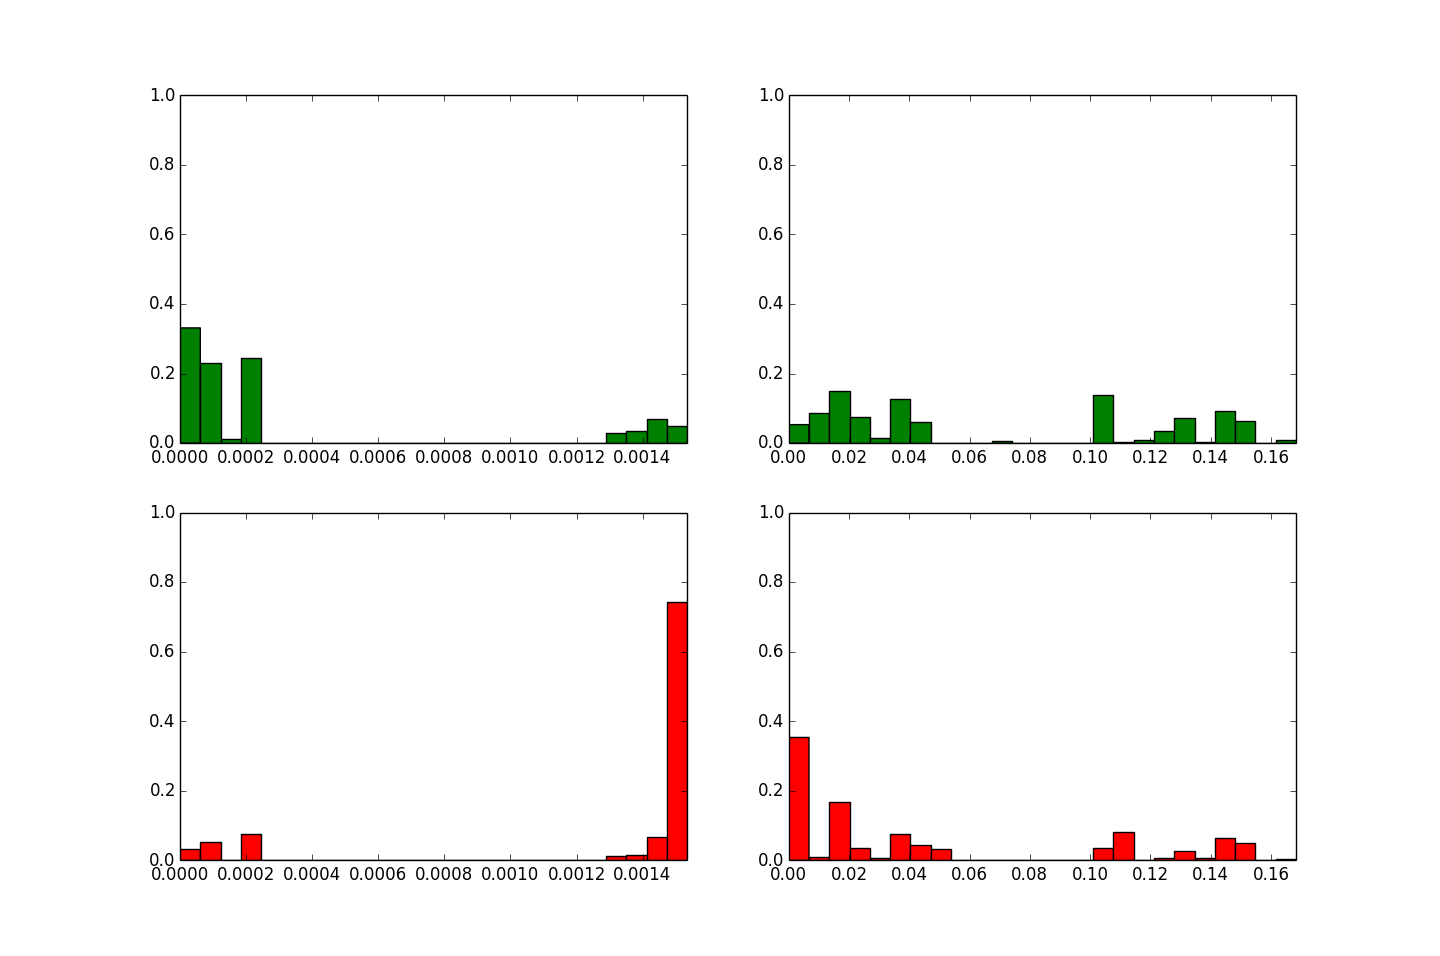
\includegraphics[width =\textwidth]{images/probabilities}
\caption{The distribution in percentages of correct (green) and incorrect (red) document links. Left hand side shows the tag probabilities and the right hand side the link probabilities.}
\label{distribution}
\end{figure}


\subsection{Threshold performance}
\begin{figure}[h!]
\begin{tabular}{cc}
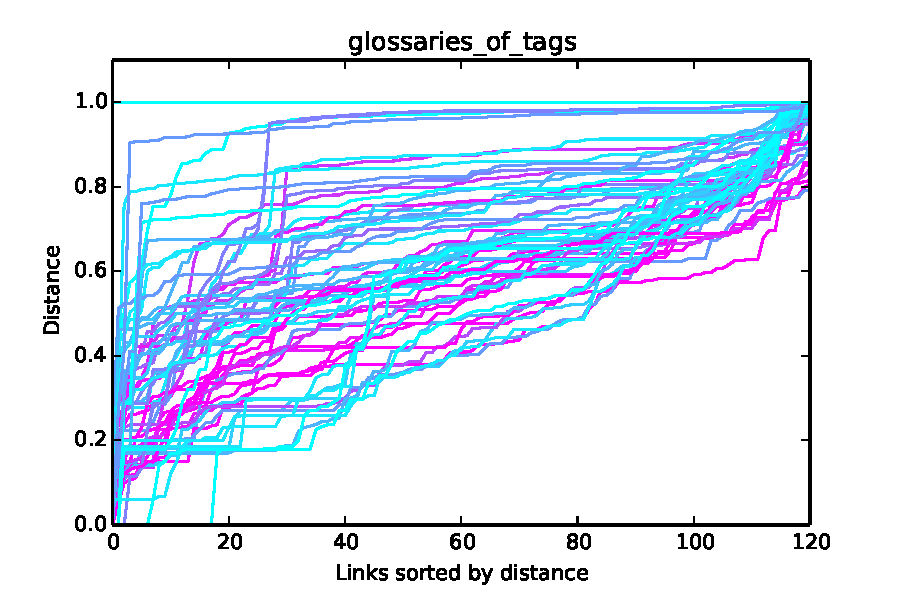
\includegraphics[width =0.5\textwidth]{images/thresh_cosine_glossaries_of_tags} 		& 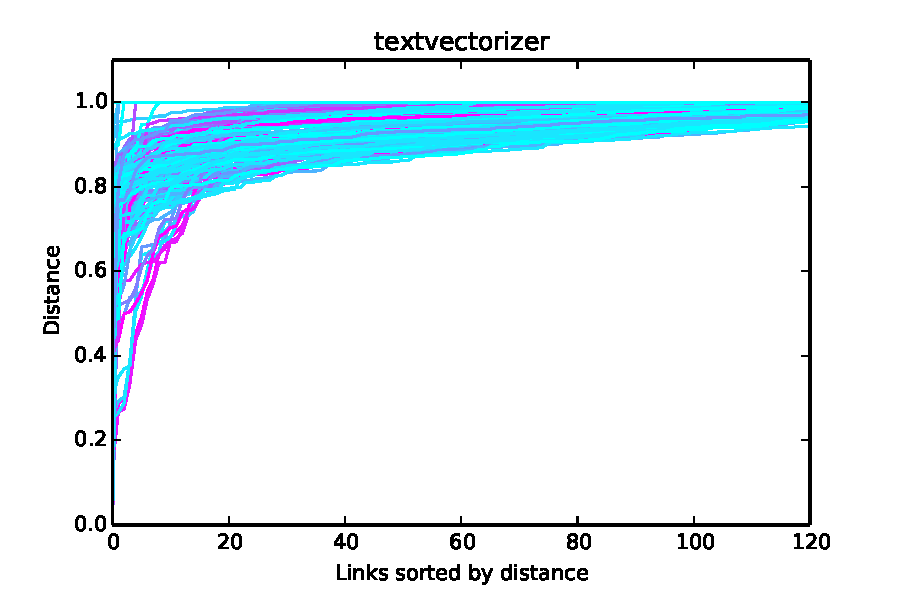
\includegraphics[width =0.5\textwidth]{images/thresh_cosine_textvectorizer} \\ \relax
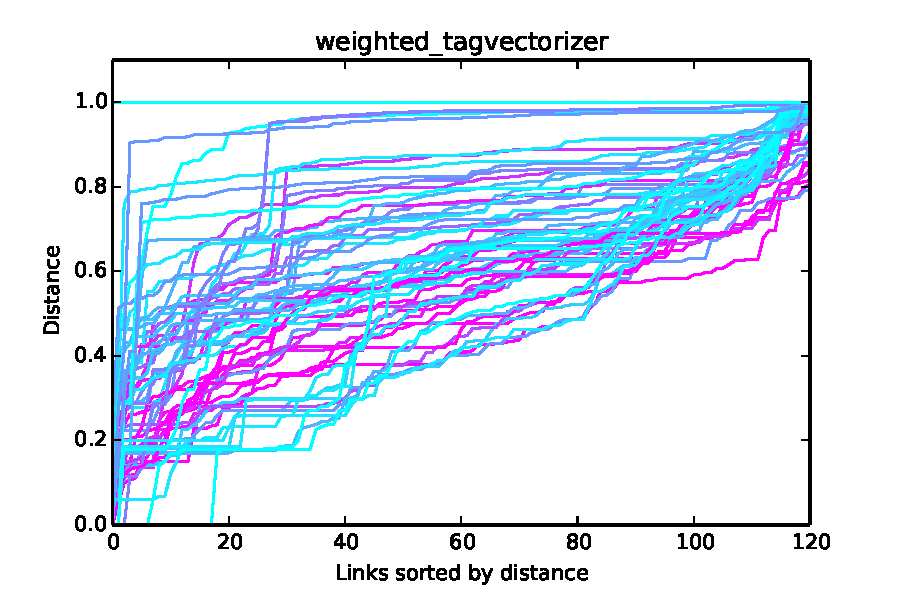
\includegraphics[width =0.5\textwidth]{images/thresh_cosine_weighted_tagvectorizer}	& 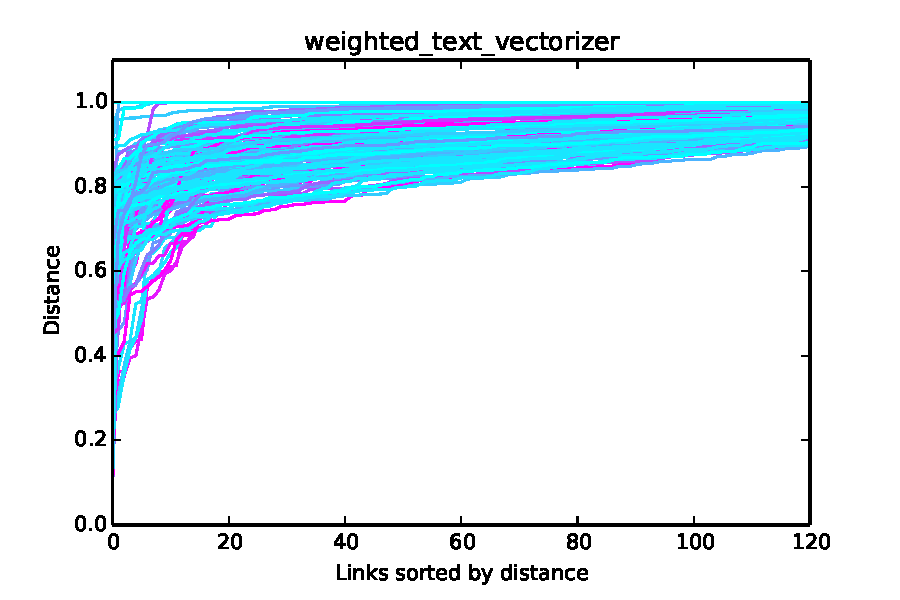
\includegraphics[width =0.5\textwidth]{images/thresh_cosine_weighted_text_vectorizer} \\ \relax
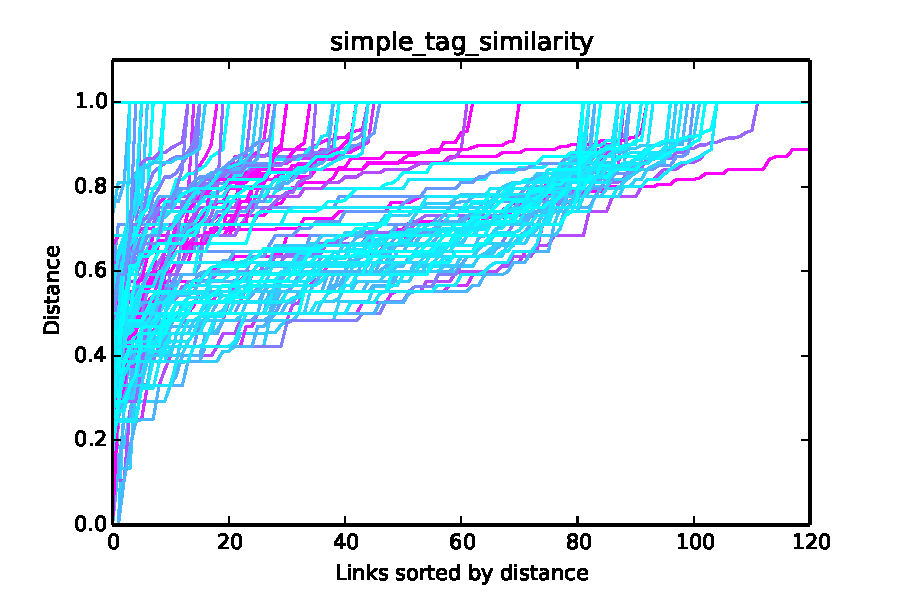
\includegraphics[width =0.5\textwidth]{images/thresh_cosine_simple_tag_similarity} 	& 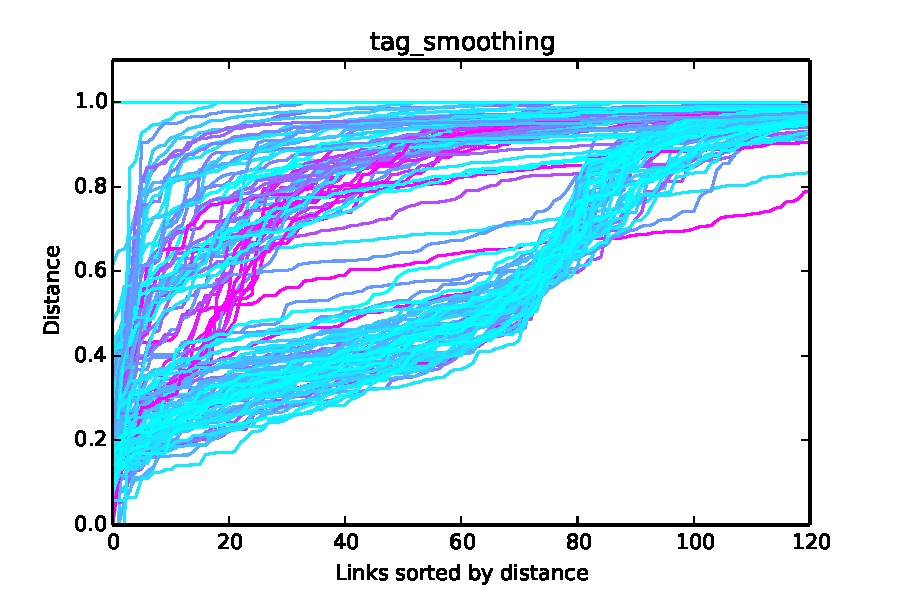
\includegraphics[width =0.5\textwidth]{images/thresh_cosine_tag_smoothing}
\end{tabular}
\caption{The sorted cosine distances of nearest neighbors and their distance for differend vectorizers. The blue purple gradient represents documents with 0 links (blue) to $\>10$ links (purple)}
\label{fig:thresholds}
\end{figure}

To evaluate the threshold, it is important to know what the result of the nearest neighbor 
algorithm is and how this relates to the way experts decide a document is relevant or 
not. Figure~\ref{fig:thresholds} shows the increase of distance for neighbors when ranked
less similar then their preceding neighbor.

Documents with little links registered in the original dataset are blueish in 
figure~\ref{fig:thresholds} and expected to have a small set of neighbors close 
by, after which the distance for the following neighbors should rise quickly. This 
general trend is visible in almost all tag vectorizers. 

Documents with more than average links registered in the original dataset are 
purplish in figure~\ref{fig:thresholds} and the neighbor distance is expected to increase
slower than the blue lines.

The results shown are very noisy, something that is to be expected from a small
human annotated dataset. However, we can detect anticipated general patterns.
Figure~\ref{fig:thresholds_differences} shows the differences between consecutive 
neighbors. In line with our understanding of expert linking, these graphs take the 
form of a long tail distribution for documents with a small amount of links.

\begin{figure}[h!]
\begin{tabular}{cc}
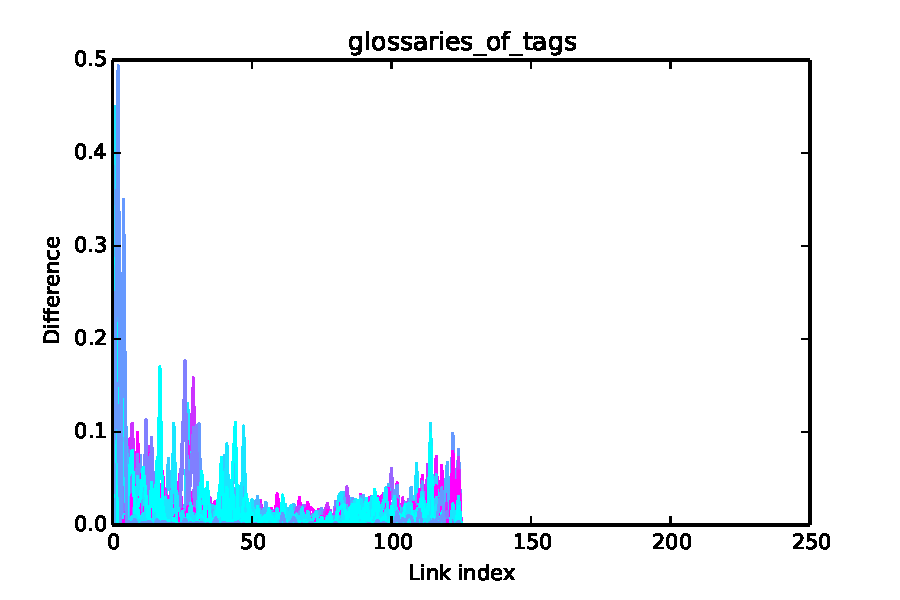
\includegraphics[width =0.5\textwidth]{images/thresh_cosine_glossaries_of_tags_distances} 		& 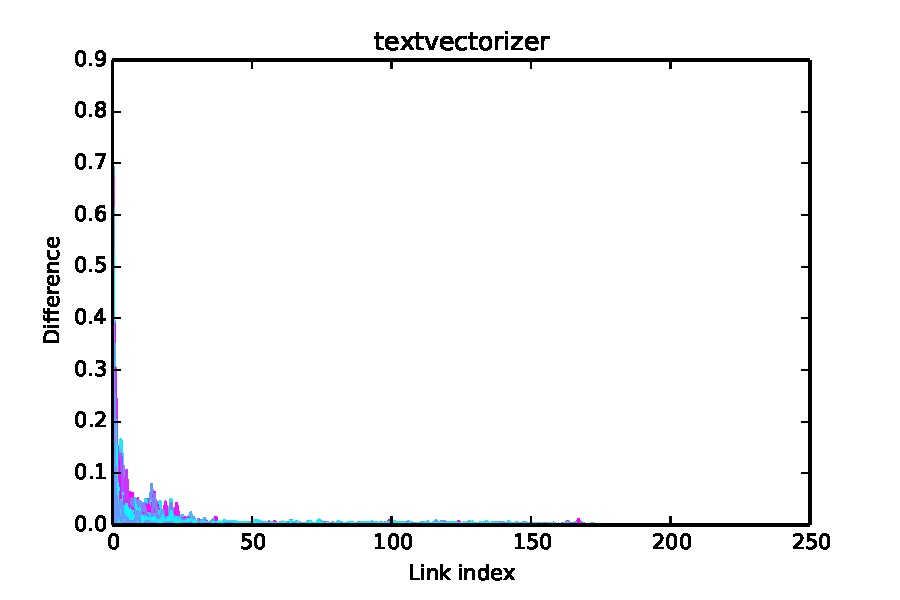
\includegraphics[width =0.5\textwidth]{images/thresh_cosine_textvectorizer_distances} \\ \relax
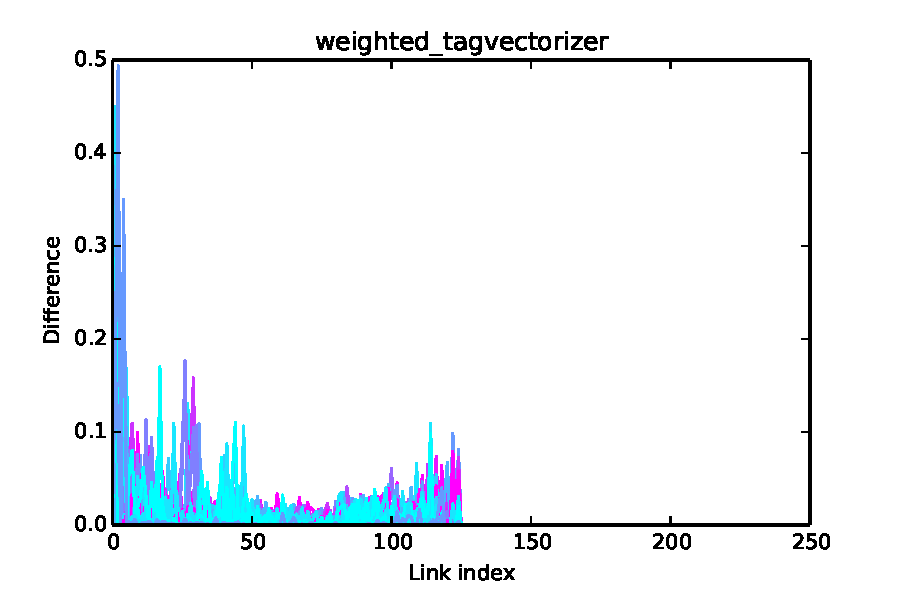
\includegraphics[width =0.5\textwidth]{images/thresh_cosine_weighted_tagvectorizer_distances}	& 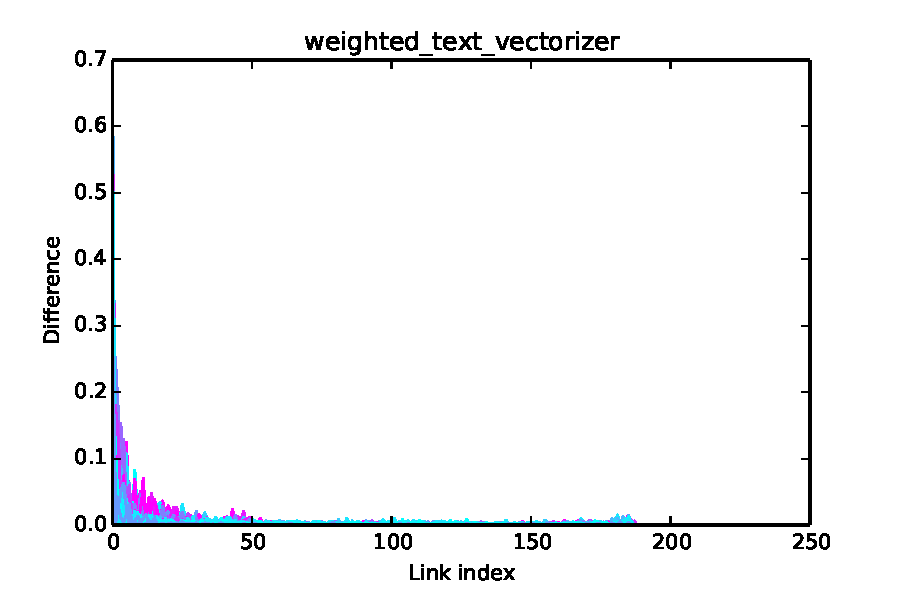
\includegraphics[width =0.5\textwidth]{images/thresh_cosine_weighted_text_vectorizer_distances} \\ \relax
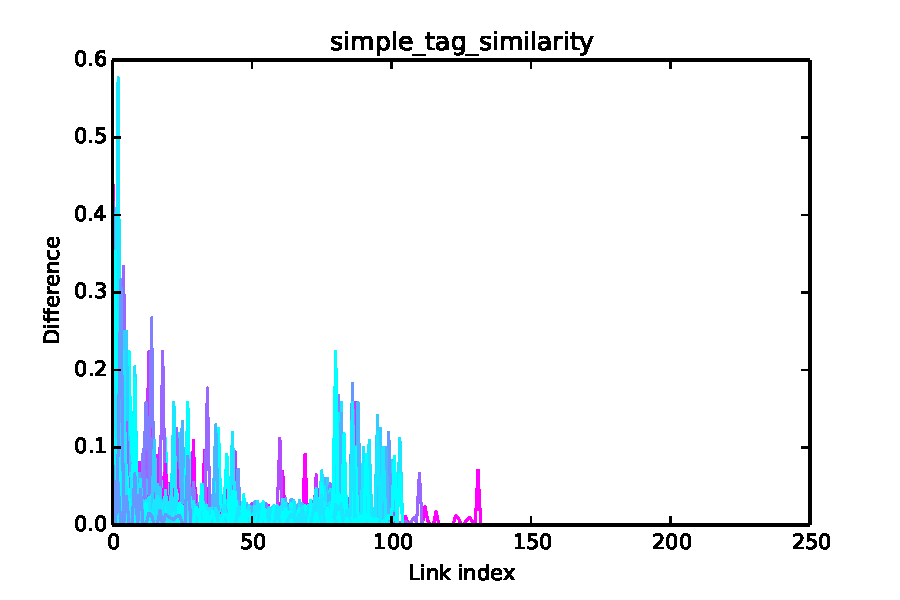
\includegraphics[width =0.5\textwidth]{images/thresh_cosine_simple_tag_similarity_distances} 	& 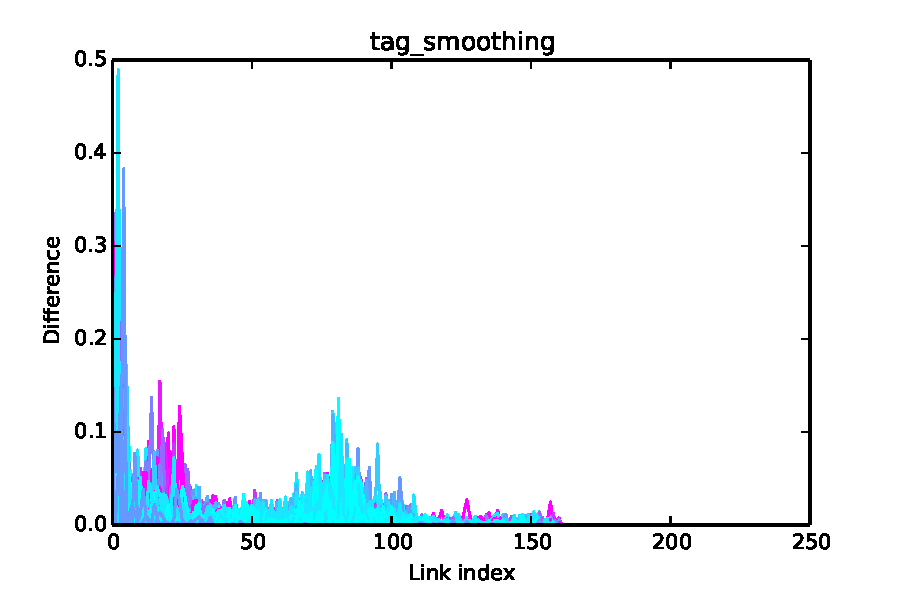
\includegraphics[width =0.5\textwidth]{images/thresh_cosine_tag_smoothing_distances}
\end{tabular}
\caption{Cosine distance differences betweeen two nearest neighbors sorted by document rank. The blue purple gradient represents documents with 0 links (blue) to $\>10$ links (purple)}
\label{fig:thresholds_differences}
\end{figure}

The above evidence suggests the nearest neighbor algorithm returns neighbours 
at distances in a similar to how experts would rate similarity. The reported decrease
of distance differences is expected and should be handled properly by the proposed
threshold calculation.

\begin{table}
\begin{tabular}{| l | l | l | l | l | l | l | l |}
\hline
THRESHOLD RECALL & Inf. &  Question &  Good Pr.& Project & Person &  Event & {\bf Average} \\
\hline
Textvectorizer & 12.05 & 39.65 & 19.64 & 20.73 & 5.21 & 21.43 & {\bf 15.66}\\
Weighted text & 14.80 & 29.82 & 19.64 & 24.37 & 5.24 & 21.43 & {\bf 15.11}\\
Simple tag & 24.14 & 20.61 & 48.21 & 30.63 & 19.49 & 26.19 & {\bf 23.26}\\
Tag smoothing & 55.56 & 20.61 & 42.86 & 34.90 & 63.33 & 33.73 & {\bf 49.56}\\
Glossaries of tags & 36.51 & 23.25 & 21.43 & 36.35 & 50.20 & 44.05 & {\bf 38.80}\\
Weighted tag & 36.52 & 23.25 & 21.43 & 36.35 & 50.20 & 44.05 & {\bf 38.80}\\
Hybrid & 24.14 & 41.40 & 48.21 & 30.63 & 20.34 & 26.19 & {\bf 27.26}\\
\hline

\hline
THRESH PRECISION & Inf. &  Question &  Good Pr.& Project & Person &  Event & {\bf Average} \\
\hline
Textvectorizer & 26.47 & 50.00 & 41.67 & 24.79 & 24.79 & 7.26 & {\bf 24.05}\\
Weighted text & 26.76 & 41.67 & 33.33 & 26.25 & 8.55 & 27.78 & {\bf 23.00}\\
Simple Tag & 28.43 & 17.54 & 62.60 & 56.25 & 10.77 & 38.89 & {\bf 23.71}\\
Tag smoothing &  0 & 0 & 0& 0 & 0 & 0 &{\bf } \\
Glossaries of tags & 25.00 & 14.47 & 37.50 & 33.18 & 17.26 & 46.67 & {\bf 22.00}\\
Weighted tag & 25.00 & 14.47 & 37.50 & 33.18 & 17.26 & 46.67 & {\bf 22.00}\\
Hybrid & 28.43 & 39.91 & 62.50 & 56.25 & 13.33 & 38.89 & {\bf 28.61}\\
\hline
\\
\hline
THRESH F1-MEASURE & Inf. &  Question &  Good Pr.& Project & Person &  Event & {\bf Average} \\
\hline
Textvectorizer & 16.56 & 44.23 & 26.70 & 22.58 & 8.61 & 10.85 & {\bf 18.97 } \\
Weighted text & 19.06 & 34.76 & 24.72 & 25.28 & 6.50 & 24.20 & {\bf 18.24 } \\
Simple tag & 26.11 & 18.95 & 54.47 & 39.66 & 13.87 & 31.30 & {\bf 23.48} \\
Tag smoothing & 0 & 0 & 0& 0 & 0 & 0 &{\bf } \\
Glossaries of tags & 29.68 & 17.84 & 27.27 & 34.69 & 25.69 & 45.32 &{\bf 28.08} \\
Weighted tag & 29.68 & 17.84 & 27.27 & 34.69 & 25.69 & 45.32 &{\bf 28.08 } \\
Hybrid &  26.11 & 40.64 & 37.46 & 39.66 & 16.11 & 31.62 &{\bf 27.91} \\
\hline
\end{tabular}

\caption{Percentage correct links per vectorizer per document type after a k-link measurement}
\label{tab:thresh_eval}
\end{table}

Knowing that the pipeline until thresholding returns sane results, the actual performance
of the proposed threshold formula is tested on the dataset. The performance of the 
automated threshold was measured for all vectorizers with the cosine metric since that one gave the overall best reuslts. Now, precision and recall are different because the threshold can 
return a different number of links than the links that are known to be correct. Table~\ref{tab:thresh_eval} 
shows the precision, recall and f1-measure for each of the vectorizers, including an unraveling for
each type of document. A comparison between this table and table \ref{klink} and table \ref{hybrid}, which were measured with the k-link metric, shows that the f1-measure of most outcomes is comparable with the k-link accuracy that was measured. However, the glossaries of tags and weighted tag vectorizer seem to have significantly better results - an f1-measure of 28.08 compared to a 18.02 k-link measurement. This seems to be caused by a much higher precision and recall for the Person type of documents. \todo{Find an example why}. 


% Conclusion
\section{Conclusion}
This report has compared six different ways (vectorizers) of converting a text
document into a vector representation and five ways of computing the distance
between these vectors. All this is done in the context of the Starfish network.
Also a method to take the knowledge from the network into account and a way to
determine the number of documents to retrieve were proposed. These combined
form a complete `pipeline' to compute and propose links to known documents for
a new document that is about to be added to the Starfish network.

The following conclusions can be drawn from the present study: firstly, the
text vectorizers perform significantly better for questions, however these do
perform badly on documents of type `person'. On documents of type `person' the
tag vectorizers do perform well. Suprisingly the simple tag vectorizer has the
best performance and is the fastest except for events. For documents of type
`events' it is recommended to use the glossaries of tags vectorizer.  Secondly
the probabilistic model of the network that is proposed is either to simplistic
or the data available is too little. In either case it might be off interest to
further investigate a similar model on a bigger data set. Lastly the method
of selecting the number of documents shows that the precision increases and
performs better than selecting a static number of documents.

The findings in this report are subject to at least three limitations. First,
the proposed solution only works for textual document and not on audio, video
which may be part of the Startfish knowledge graph. Secondly, the data set
that was used during investigation is rather small and may not be representation
of a real life data set. Lastly due to the small training network no cross-validation
was performed which may result in an overfit to the data.

Whilst this study is based on only a small network of documents taken together
these findings do show that the chosen solution is capable of recommending
links between documents with a certainty far above the guessing level. It is
now up to the client to choose if a precision of 45.09\% is good enough to
let the user select a document to link.



% MUCH FUTURE WORK!
\section{Future Work \& Recommendations}
Latent dirichlet allocation because tags in dataset are not so good.

Also create incoming links




% Marshall Matters
\bibliographystyle{apalike}
\bibliography{references.bib}


\end{document}
